\subsubsection{Rouge}
Rouge is a metric proposed to compare the quality of summaries with gold standard summaries \cite{lin2004rouge}. It works by counting the number of overlapping n-grams between the generated and the reference summary. Commonly used are unigrams, bigrams and longest n-grams, called ROUGE-1, ROUGE-2 and ROUGE-L respectively. We apply ROUGE-2 to our summaries with each of the other groups summaries as references. With $N$ describing the topics and $M$ describing the groups we calculate the score for group $a$ as:
$$\frac{1}{NM} \sum^N_{n} \sum^M_{m\neq a} ROUGE(\hat{s}_{n,a}, s_{n,m}) $$
We find that ROUGE-2 performs the best, as the spearman correlation between the topicwise ROUGE-2 and the manual score was $0.15$, while it was only $0.04$ and $0.08$ for ROUGE-1 and ROUGE-L respectively.

\begin{figure}[!ht]
	\centering
	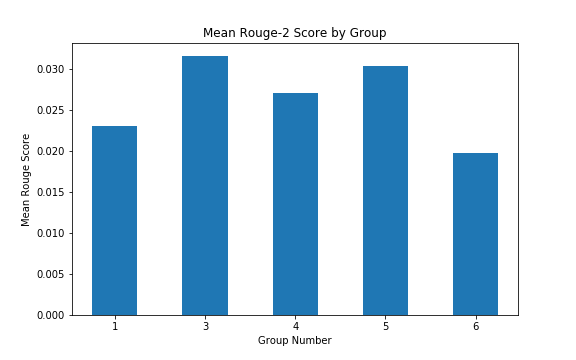
\includegraphics[width=0.55\linewidth]{../evaluation/meanrouge.png}
	\caption{Groups performance by ROUGE-2}
	\label{fig:rouge}
\end{figure}

As can be seen in figure \ref{fig:rouge} our summaries were on par with group 6, but behind the other three groups with a significant gap. Keep in mind that ROUGE measures the similarity, but similarity to the other groups might not always be indicative of a good summary. 